% Options for packages loaded elsewhere
\PassOptionsToPackage{unicode}{hyperref}
\PassOptionsToPackage{hyphens}{url}
%
\documentclass[
  11pt,
]{article}
\usepackage[]{mathpazo}
\usepackage{amsmath}
\usepackage{ifxetex,ifluatex}
\ifnum 0\ifxetex 1\fi\ifluatex 1\fi=0 % if pdftex
  \usepackage[T1]{fontenc}
  \usepackage[utf8]{inputenc}
  \usepackage{textcomp} % provide euro and other symbols
  \usepackage{amssymb}
\else % if luatex or xetex
  \usepackage{unicode-math}
  \defaultfontfeatures{Scale=MatchLowercase}
  \defaultfontfeatures[\rmfamily]{Ligatures=TeX,Scale=1}
\fi
% Use upquote if available, for straight quotes in verbatim environments
\IfFileExists{upquote.sty}{\usepackage{upquote}}{}
\IfFileExists{microtype.sty}{% use microtype if available
  \usepackage[]{microtype}
  \UseMicrotypeSet[protrusion]{basicmath} % disable protrusion for tt fonts
}{}
\makeatletter
\@ifundefined{KOMAClassName}{% if non-KOMA class
  \IfFileExists{parskip.sty}{%
    \usepackage{parskip}
  }{% else
    \setlength{\parindent}{0pt}
    \setlength{\parskip}{6pt plus 2pt minus 1pt}}
}{% if KOMA class
  \KOMAoptions{parskip=half}}
\makeatother
\usepackage{xcolor}
\IfFileExists{xurl.sty}{\usepackage{xurl}}{} % add URL line breaks if available
\IfFileExists{bookmark.sty}{\usepackage{bookmark}}{\usepackage{hyperref}}
\hypersetup{
  pdftitle={Conditional Probability and Volatility Clustering},
  pdfauthor={Patrick Hénaff},
  hidelinks,
  pdfcreator={LaTeX via pandoc}}
\urlstyle{same} % disable monospaced font for URLs
\usepackage[margin=1in]{geometry}
\usepackage{color}
\usepackage{fancyvrb}
\newcommand{\VerbBar}{|}
\newcommand{\VERB}{\Verb[commandchars=\\\{\}]}
\DefineVerbatimEnvironment{Highlighting}{Verbatim}{commandchars=\\\{\}}
% Add ',fontsize=\small' for more characters per line
\usepackage{framed}
\definecolor{shadecolor}{RGB}{248,248,248}
\newenvironment{Shaded}{\begin{snugshade}}{\end{snugshade}}
\newcommand{\AlertTok}[1]{\textcolor[rgb]{0.94,0.16,0.16}{#1}}
\newcommand{\AnnotationTok}[1]{\textcolor[rgb]{0.56,0.35,0.01}{\textbf{\textit{#1}}}}
\newcommand{\AttributeTok}[1]{\textcolor[rgb]{0.77,0.63,0.00}{#1}}
\newcommand{\BaseNTok}[1]{\textcolor[rgb]{0.00,0.00,0.81}{#1}}
\newcommand{\BuiltInTok}[1]{#1}
\newcommand{\CharTok}[1]{\textcolor[rgb]{0.31,0.60,0.02}{#1}}
\newcommand{\CommentTok}[1]{\textcolor[rgb]{0.56,0.35,0.01}{\textit{#1}}}
\newcommand{\CommentVarTok}[1]{\textcolor[rgb]{0.56,0.35,0.01}{\textbf{\textit{#1}}}}
\newcommand{\ConstantTok}[1]{\textcolor[rgb]{0.00,0.00,0.00}{#1}}
\newcommand{\ControlFlowTok}[1]{\textcolor[rgb]{0.13,0.29,0.53}{\textbf{#1}}}
\newcommand{\DataTypeTok}[1]{\textcolor[rgb]{0.13,0.29,0.53}{#1}}
\newcommand{\DecValTok}[1]{\textcolor[rgb]{0.00,0.00,0.81}{#1}}
\newcommand{\DocumentationTok}[1]{\textcolor[rgb]{0.56,0.35,0.01}{\textbf{\textit{#1}}}}
\newcommand{\ErrorTok}[1]{\textcolor[rgb]{0.64,0.00,0.00}{\textbf{#1}}}
\newcommand{\ExtensionTok}[1]{#1}
\newcommand{\FloatTok}[1]{\textcolor[rgb]{0.00,0.00,0.81}{#1}}
\newcommand{\FunctionTok}[1]{\textcolor[rgb]{0.00,0.00,0.00}{#1}}
\newcommand{\ImportTok}[1]{#1}
\newcommand{\InformationTok}[1]{\textcolor[rgb]{0.56,0.35,0.01}{\textbf{\textit{#1}}}}
\newcommand{\KeywordTok}[1]{\textcolor[rgb]{0.13,0.29,0.53}{\textbf{#1}}}
\newcommand{\NormalTok}[1]{#1}
\newcommand{\OperatorTok}[1]{\textcolor[rgb]{0.81,0.36,0.00}{\textbf{#1}}}
\newcommand{\OtherTok}[1]{\textcolor[rgb]{0.56,0.35,0.01}{#1}}
\newcommand{\PreprocessorTok}[1]{\textcolor[rgb]{0.56,0.35,0.01}{\textit{#1}}}
\newcommand{\RegionMarkerTok}[1]{#1}
\newcommand{\SpecialCharTok}[1]{\textcolor[rgb]{0.00,0.00,0.00}{#1}}
\newcommand{\SpecialStringTok}[1]{\textcolor[rgb]{0.31,0.60,0.02}{#1}}
\newcommand{\StringTok}[1]{\textcolor[rgb]{0.31,0.60,0.02}{#1}}
\newcommand{\VariableTok}[1]{\textcolor[rgb]{0.00,0.00,0.00}{#1}}
\newcommand{\VerbatimStringTok}[1]{\textcolor[rgb]{0.31,0.60,0.02}{#1}}
\newcommand{\WarningTok}[1]{\textcolor[rgb]{0.56,0.35,0.01}{\textbf{\textit{#1}}}}
\usepackage{longtable,booktabs}
\usepackage{calc} % for calculating minipage widths
% Correct order of tables after \paragraph or \subparagraph
\usepackage{etoolbox}
\makeatletter
\patchcmd\longtable{\par}{\if@noskipsec\mbox{}\fi\par}{}{}
\makeatother
% Allow footnotes in longtable head/foot
\IfFileExists{footnotehyper.sty}{\usepackage{footnotehyper}}{\usepackage{footnote}}
\makesavenoteenv{longtable}
\usepackage{graphicx}
\makeatletter
\def\maxwidth{\ifdim\Gin@nat@width>\linewidth\linewidth\else\Gin@nat@width\fi}
\def\maxheight{\ifdim\Gin@nat@height>\textheight\textheight\else\Gin@nat@height\fi}
\makeatother
% Scale images if necessary, so that they will not overflow the page
% margins by default, and it is still possible to overwrite the defaults
% using explicit options in \includegraphics[width, height, ...]{}
\setkeys{Gin}{width=\maxwidth,height=\maxheight,keepaspectratio}
% Set default figure placement to htbp
\makeatletter
\def\fps@figure{htbp}
\makeatother
\setlength{\emergencystretch}{3em} % prevent overfull lines
\providecommand{\tightlist}{%
  \setlength{\itemsep}{0pt}\setlength{\parskip}{0pt}}
\setcounter{secnumdepth}{5}
\linespread{1.05}
\usepackage[utf8]{inputenc}
\usepackage{amsthm}
\usepackage{xfrac}
\usepackage{float}
\ifluatex
  \usepackage{selnolig}  % disable illegal ligatures
\fi
\newlength{\cslhangindent}
\setlength{\cslhangindent}{1.5em}
\newlength{\csllabelwidth}
\setlength{\csllabelwidth}{3em}
\newenvironment{CSLReferences}[2] % #1 hanging-ident, #2 entry spacing
 {% don't indent paragraphs
  \setlength{\parindent}{0pt}
  % turn on hanging indent if param 1 is 1
  \ifodd #1 \everypar{\setlength{\hangindent}{\cslhangindent}}\ignorespaces\fi
  % set entry spacing
  \ifnum #2 > 0
  \setlength{\parskip}{#2\baselineskip}
  \fi
 }%
 {}
\usepackage{calc}
\newcommand{\CSLBlock}[1]{#1\hfill\break}
\newcommand{\CSLLeftMargin}[1]{\parbox[t]{\csllabelwidth}{#1}}
\newcommand{\CSLRightInline}[1]{\parbox[t]{\linewidth - \csllabelwidth}{#1}\break}
\newcommand{\CSLIndent}[1]{\hspace{\cslhangindent}#1}

\title{Conditional Probability and Volatility Clustering}
\author{Patrick Hénaff}
\date{Feb 2021}

\begin{document}
\maketitle

The purpose of this note is to reproduce and comment some results on the conditional distribution of returns, presented by K. Chen \emph{et al} in (Chen et al., 2008). We provide the code and data to reproduce the calculations presented in the paper, and are able to reproduce its figures. We however show that the advocated model does not fully account for the ``volatility clustering,'' an important stylized fact of financial time series.

\hypertarget{sec:fts}{%
\section{Characteristics of Financial Time Series}\label{sec:fts}}

The characteristic features of financial time series have been
extensively documented (Cont, 2001). As mentioned, a distribution of
returns with "fat tails", and volatility clustering are the key
aspects of these series. (Chen et al., 2008) shows that for many financial time
series, the return at any time scale is, beyond some threshold,
distributed according to a power law. The parameters of this power law
depend upon the magnitude of return in the previous period (this is the
volatility clustering feature). Moreover, when return is scaled
conditionally to the magnitude of the previous period return, the
distribution is found to follow a universal form, asymmetrical and with
fat tails.

Let \(\{r\}\) be a series of returns, computed at intervals \(\Delta t\).
Following Chen's notation, the values of \(r\) are binned according to
\(r_p\), the magnitude of return in the previous period. The standard
deviation of each bin is \(w(r_p)\). the distribution of return,
conditional upon the magnitude of the previous return, can be expressed
as:
\begin{equation}
P(r | r_p) = \frac{1}{w(r_p)} f \left( \frac{r}{w(r_p)} \right)
\label{eq:cond-dist}
\end{equation}
with:

\begin{description}
\item[\(r\)]
return over a time interval \(\Delta t\)
\item[\(r_p\)]
absolute value of return in the previous period
\item[\(w(r_p)\)]
standard deviation of \(r\) in the bin defined by \(r_p\)
\item[\(f()\)]
distribution of return, conditionally normalized
\end{description}

It follows that the joint distribution of \(r\) and \(r_p\) given by
(\ref{eq:cond-dist}) captures both the features described by \(f()\)
(fat tails, asymmetry) and the conditional variance (volatility
clustering).

Numerous studies (Gopikrishnan et al., 1998) have
documented that the cumulative distribution of returns, beyond some
threshold, can be described by a power law, that is, in the notation of
(\ref{eq:cond-dist}):

\begin{equation}
f \left( x \right) = \frac{\alpha-1}{x_{\mbox{min}}} \left( \frac{x}{x_{\mbox{min}}} \right)^{-\alpha}, \ \ x>x_{\mbox{min}}
\label{eq:power-law}
\end{equation}

Chen et al. (2008, p. 2) notes that the distribution of scaled conditional
return, \(P(r | r_p)\) "collapses to a universal curve", and this can
indeed be observed on some time series. Following Chen, we consider a
long series of the Dow Jones Industrial Average, from 1900 to 2004,
provided by Williamson (2013). The series is sampled every \(T=2\) days, and
we use 8 bins of equal size to partition \(r_p\).

\begin{Shaded}
\begin{Highlighting}[]
\CommentTok{\# number of bins}
\NormalTok{nb }\OtherTok{\textless{}{-}} \DecValTok{8}
\NormalTok{ticker }\OtherTok{\textless{}{-}} \StringTok{\textquotesingle{}djia\textquotesingle{}}
\NormalTok{r.djia }\OtherTok{\textless{}{-}} \FunctionTok{get.ts}\NormalTok{(ticker, }\AttributeTok{calc=}\StringTok{\textquotesingle{}return\textquotesingle{}}\NormalTok{)}
\NormalTok{ticker }\OtherTok{\textless{}{-}} \StringTok{\textquotesingle{}qqq\textquotesingle{}}
\NormalTok{r.QQQ }\OtherTok{\textless{}{-}} \FunctionTok{get.ts}\NormalTok{(ticker, }\AttributeTok{calc=}\StringTok{\textquotesingle{}return\textquotesingle{}}\NormalTok{)}
\end{Highlighting}
\end{Shaded}

The next function allocate observations \(r_t\) into \(nb\) bins, conditional upon the value of \(|r_{t-1}|\).

\begin{Shaded}
\begin{Highlighting}[]
\NormalTok{bins.djia }\OtherTok{\textless{}{-}} \FunctionTok{make.bins}\NormalTok{(r.djia, }\AttributeTok{NBIN=}\NormalTok{nb, }\AttributeTok{model=}\StringTok{\textquotesingle{}abs\textquotesingle{}}\NormalTok{, params)}
\NormalTok{bins.QQQ }\OtherTok{\textless{}{-}} \FunctionTok{make.bins}\NormalTok{(r.QQQ, }\AttributeTok{NBIN=}\NormalTok{nb, }\AttributeTok{model=}\StringTok{\textquotesingle{}abs\textquotesingle{}}\NormalTok{, params)}
\end{Highlighting}
\end{Shaded}

Following the article in reference, we plot the conditional density of return for each bin. The width of the density is positively correlated to the magnitude of \(|r_{t-1}|\),
although the pattern is more visible for QQQ (as reported in the paper) as for, for example, for DJIA. This is illustrated in the following two figures.

\begin{Shaded}
\begin{Highlighting}[]
\FunctionTok{par}\NormalTok{(}\AttributeTok{mar=}\FunctionTok{c}\NormalTok{(}\DecValTok{4}\NormalTok{,}\DecValTok{4}\NormalTok{,}\FloatTok{0.1}\NormalTok{,}\FloatTok{0.1}\NormalTok{))}
\FunctionTok{plot.conditional.r}\NormalTok{(}\AttributeTok{r=}\NormalTok{r.QQQ, }\AttributeTok{bins=}\NormalTok{bins.QQQ, }\AttributeTok{ticker=}\StringTok{\textquotesingle{}QQQ\textquotesingle{}}\NormalTok{,}\AttributeTok{NBIN=}\NormalTok{nb)}
\FunctionTok{plot.conditional.r}\NormalTok{(}\AttributeTok{r=}\NormalTok{r.djia, }\AttributeTok{bins=}\NormalTok{bins.djia, }\AttributeTok{ticker=}\StringTok{\textquotesingle{}DJIA\textquotesingle{}}\NormalTok{,}\AttributeTok{NBIN=}\NormalTok{nb)}
\end{Highlighting}
\end{Shaded}

\begin{figure}[H]
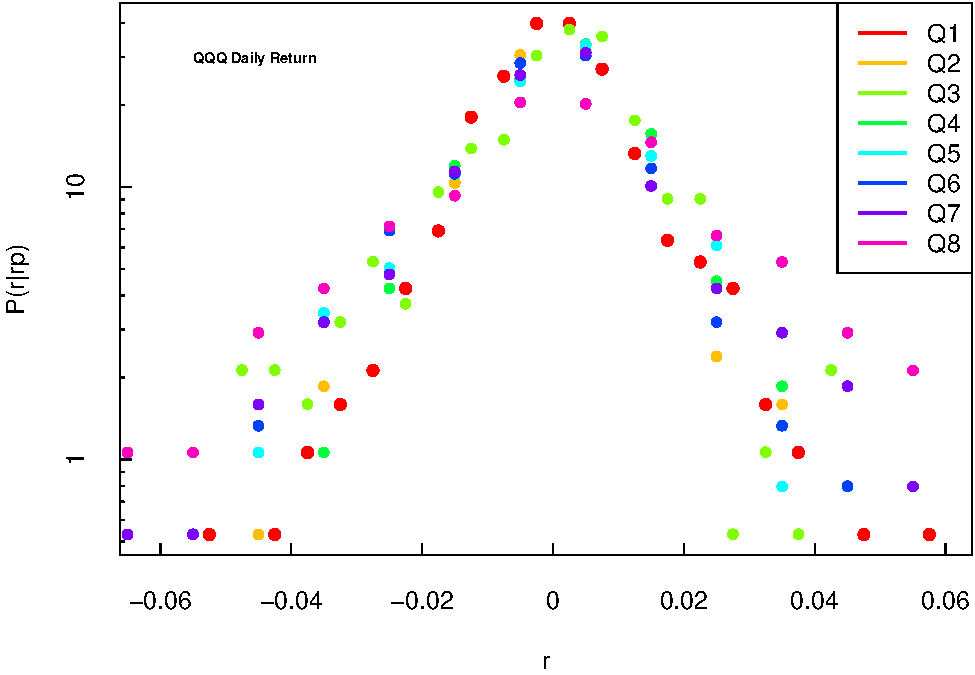
\includegraphics[width=0.5\linewidth]{figs/condist-plot-1} 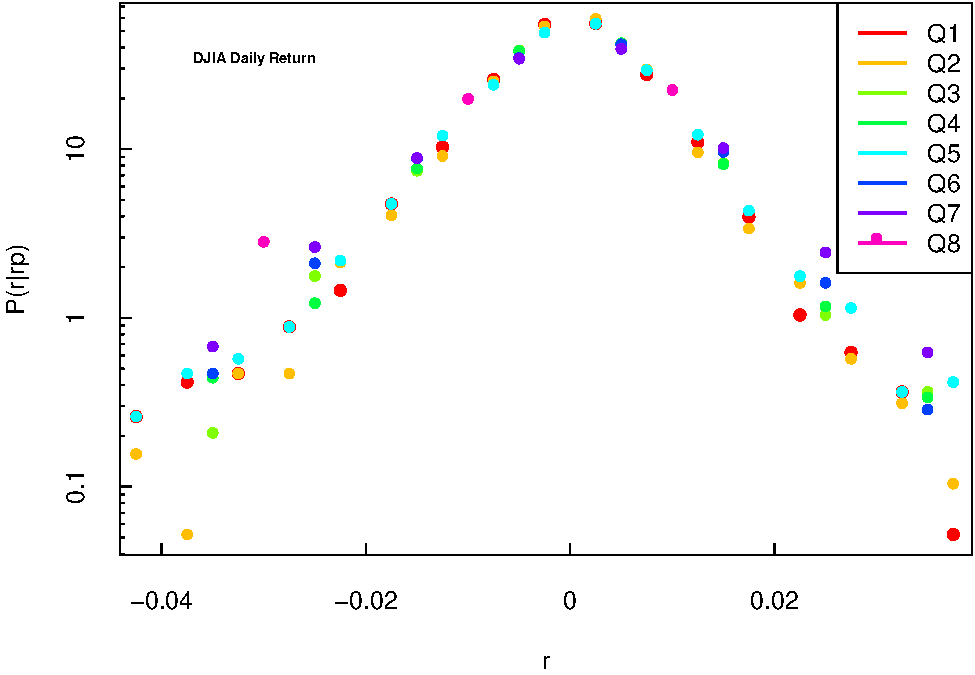
\includegraphics[width=0.5\linewidth]{figs/condist-plot-2} \caption{Conditional density of QQQ and DJIA return. $r$ is partitioned in 8 bins of equal size, according to the absolute value of return in the previous period.}\label{fig:condist-plot}
\end{figure}

Using the estimation
method introduced by Clauset et al. (2009), and considering each bin separately,
we fit the tail distribution to a power law. The parameters
\(\alpha_{\text{min}}\) and \(\alpha\) specific to each bin are reported in
Figure \ref{fig:powerlawplot}.
The results are consistent with the ones reported by Chen \emph{et al.}

\begin{Shaded}
\begin{Highlighting}[]
\NormalTok{params }\OtherTok{=} \FunctionTok{list}\NormalTok{(}\AttributeTok{lambda=}\FloatTok{0.94}\NormalTok{, }\AttributeTok{nb.init=}\DecValTok{250}\NormalTok{)}
\FunctionTok{plot.cum.cond.r}\NormalTok{(}\AttributeTok{r=}\NormalTok{r.djia, }\AttributeTok{bins=}\NormalTok{bins.djia, }\AttributeTok{ticker=}\StringTok{\textquotesingle{}djia\textquotesingle{}}\NormalTok{, }\AttributeTok{sgn=}\StringTok{\textquotesingle{}all\textquotesingle{}}\NormalTok{,}
\AttributeTok{NBIN=}\NormalTok{nb, }\AttributeTok{model=}\StringTok{\textquotesingle{}abs\textquotesingle{}}\NormalTok{, }\AttributeTok{params=}\NormalTok{params)}
\end{Highlighting}
\end{Shaded}

\begin{figure}[H]
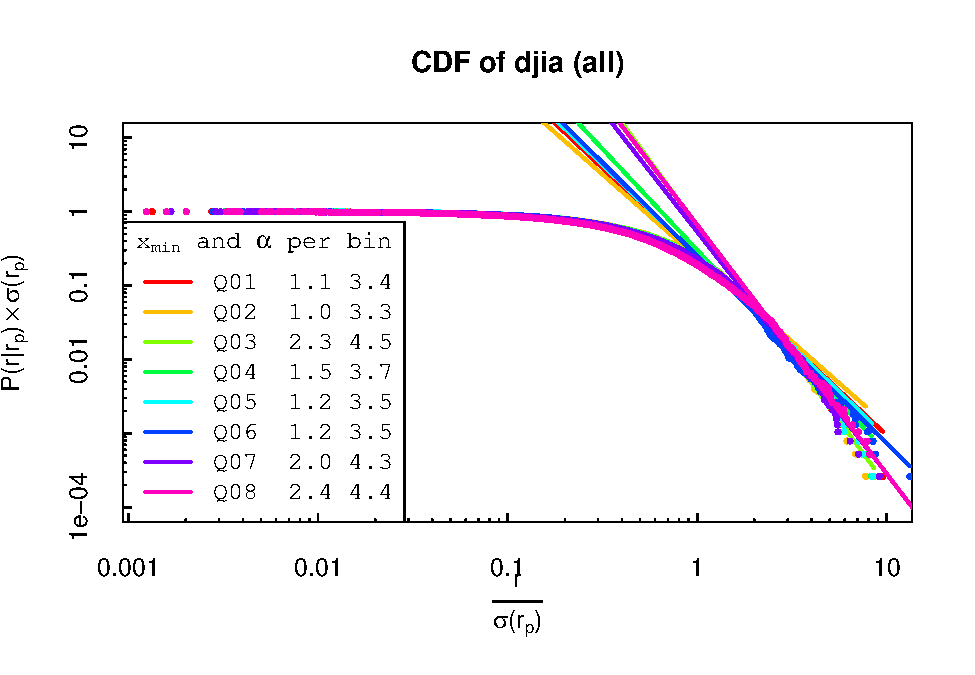
\includegraphics[width=0.7\linewidth,height=0.7\textheight]{figs/powerlawplot-1} \caption{Cumulative density of DJIA return. $r$ is partitioned in 8 bins of equal size, according to the absolute value of return in the previous period. For each bin, the inserted table reports $x_{\text{min}}$ and $\alpha$.}\label{fig:powerlawplot}
\end{figure}

However, the claim should perhaps not be taken literally: it is not
hard to identify time series that do not exhibit a "collapse to a
universal curve". Figure \ref{fig:bnp2}, among many examples, displays the results of the
same calculation, applied to the BNP (BNP.PA) stock, using daily close
prices from 2000 to 2013. The conditional scaled tail return for the
first bin (the bin corresponding to returns of small magnitude in the
previous time interval) shows a marked difference from the distributions
of the other bins.

\begin{Shaded}
\begin{Highlighting}[]
\NormalTok{ticker }\OtherTok{\textless{}{-}} \StringTok{\textquotesingle{}bnp\textquotesingle{}}
\NormalTok{r.bnp }\OtherTok{\textless{}{-}} \FunctionTok{get.ts}\NormalTok{(ticker, }\AttributeTok{calc=}\StringTok{\textquotesingle{}return\textquotesingle{}}\NormalTok{)}
\NormalTok{bins }\OtherTok{\textless{}{-}} \FunctionTok{make.bins}\NormalTok{(r.bnp, }\AttributeTok{NBIN=}\NormalTok{nb, }\AttributeTok{model=}\StringTok{\textquotesingle{}abs\textquotesingle{}}\NormalTok{, params)}
\end{Highlighting}
\end{Shaded}

\begin{Shaded}
\begin{Highlighting}[]
\FunctionTok{plot.cum.cond.r}\NormalTok{(}\AttributeTok{r=}\NormalTok{r.bnp, }\AttributeTok{bins=}\NormalTok{bins, }\AttributeTok{ticker=}\NormalTok{ticker, }\AttributeTok{sgn=}\StringTok{\textquotesingle{}all\textquotesingle{}}\NormalTok{,}
\AttributeTok{NBIN=}\NormalTok{nb, }\AttributeTok{model=}\StringTok{\textquotesingle{}abs\textquotesingle{}}\NormalTok{, }\AttributeTok{params=}\NormalTok{params)}
\end{Highlighting}
\end{Shaded}

\begin{figure}[H]
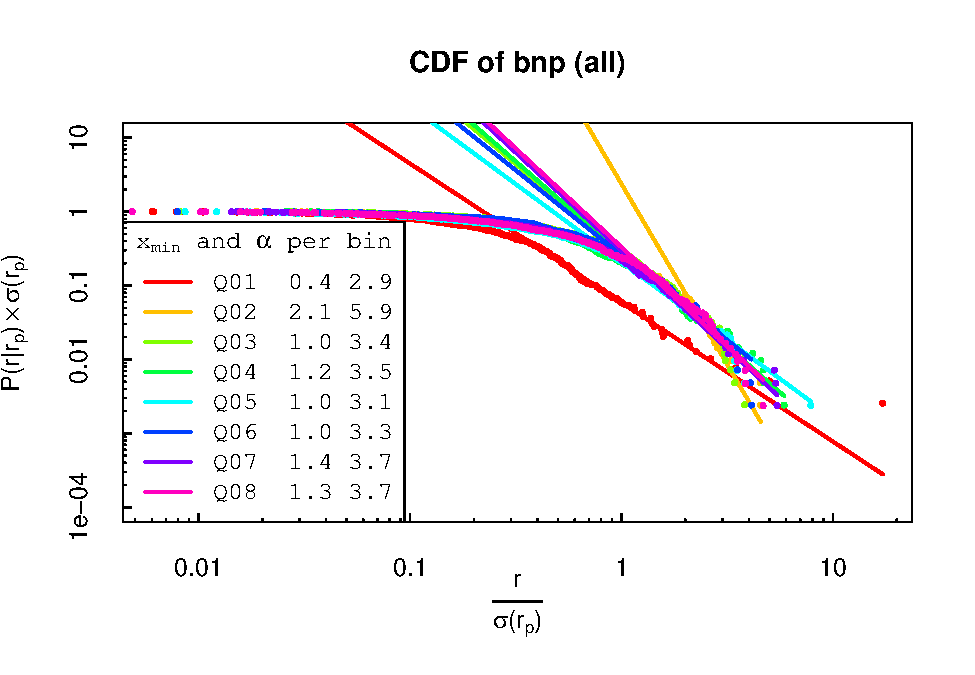
\includegraphics[width=0.7\linewidth,height=0.7\textheight]{figs/bnp2-1} \caption{CDF of BNP (BNP.PA) return. The conditional scaled tail return for the first bin (the bin corresponding to returns of small magnitude in the previous time interval) shows a marked difference from the distributions of the other bins.}\label{fig:bnp2}
\end{figure}

\hypertarget{relationship-between-the-scaling-factor-and-r_p}{%
\subsection{\texorpdfstring{Relationship between the scaling factor and \(|r_p|\)}{Relationship between the scaling factor and \textbar r\_p\textbar{}}}\label{relationship-between-the-scaling-factor-and-r_p}}

For \(r_p\) sufficiently large, there is an apparent linear relationship between \(r_p\) and \(\sigma(r_p)\). This observation is consistent with volatility clustering, and is illustrated by the following calculation, which reproduces Figure 2 of Chen's paper.

\begin{Shaded}
\begin{Highlighting}[]
\NormalTok{ticker }\OtherTok{\textless{}{-}} \StringTok{\textquotesingle{}qqq\textquotesingle{}}
\NormalTok{p }\OtherTok{\textless{}{-}} \FunctionTok{get.ts}\NormalTok{(ticker, }\AttributeTok{calc=}\StringTok{\textquotesingle{}price\textquotesingle{}}\NormalTok{)}
\NormalTok{nb }\OtherTok{\textless{}{-}} \DecValTok{8}

\CommentTok{\# sample at T=2}
\NormalTok{indx }\OtherTok{\textless{}{-}} \FunctionTok{seq}\NormalTok{(}\DecValTok{1}\NormalTok{, }\FunctionTok{length}\NormalTok{(p), }\AttributeTok{by=}\DecValTok{2}\NormalTok{)}
\NormalTok{r}\FloatTok{.2} \OtherTok{\textless{}{-}} \FunctionTok{returns}\NormalTok{(p[indx,])}
\CommentTok{\# sample at T=20}
\NormalTok{indx }\OtherTok{\textless{}{-}} \FunctionTok{seq}\NormalTok{(}\DecValTok{1}\NormalTok{, }\FunctionTok{length}\NormalTok{(p), }\AttributeTok{by=}\DecValTok{20}\NormalTok{)}
\NormalTok{r}\FloatTok{.20} \OtherTok{\textless{}{-}} \FunctionTok{returns}\NormalTok{(p[indx,])}
\end{Highlighting}
\end{Shaded}

\begin{Shaded}
\begin{Highlighting}[]
\FunctionTok{plot.scaling.factor}\NormalTok{(}\AttributeTok{plot.type=}\StringTok{\textquotesingle{}plot\textquotesingle{}}\NormalTok{, }\AttributeTok{r=}\NormalTok{r}\FloatTok{.2}\NormalTok{, }\AttributeTok{NBIN=}\NormalTok{nb, }\AttributeTok{type=}\StringTok{\textquotesingle{}b\textquotesingle{}}\NormalTok{,}
                    \AttributeTok{pch=}\DecValTok{16}\NormalTok{, }\AttributeTok{forcexlim=}\FunctionTok{c}\NormalTok{(}\DecValTok{0}\NormalTok{,.}\DecValTok{01}\NormalTok{),}
                    \AttributeTok{forceylim=}\FunctionTok{c}\NormalTok{(.}\DecValTok{0}\NormalTok{, .}\DecValTok{01}\NormalTok{), }
                    \AttributeTok{main=}\FunctionTok{TeX}\NormalTok{(}\StringTok{\textquotesingle{}$}\SpecialCharTok{\textbackslash{}\textbackslash{}}\StringTok{sigma(r\_p)$ as a function of $r\_p\textquotesingle{}}\NormalTok{))}

\FunctionTok{plot.scaling.factor}\NormalTok{(}\AttributeTok{plot.type=}\StringTok{\textquotesingle{}lines\textquotesingle{}}\NormalTok{, }\AttributeTok{r=}\NormalTok{r}\FloatTok{.20}\NormalTok{, }\AttributeTok{NBIN=}\NormalTok{nb, }
                    \AttributeTok{type=}\StringTok{\textquotesingle{}b\textquotesingle{}}\NormalTok{, }\AttributeTok{pch=}\DecValTok{1}\NormalTok{)}
\NormalTok{labels }\OtherTok{\textless{}{-}} \FunctionTok{c}\NormalTok{(}\StringTok{\textquotesingle{}T=2\textquotesingle{}}\NormalTok{, }\StringTok{\textquotesingle{}T=20\textquotesingle{}}\NormalTok{)}
\FunctionTok{legend}\NormalTok{(}\StringTok{\textquotesingle{}topleft\textquotesingle{}}\NormalTok{, labels, }\AttributeTok{lty=}\FunctionTok{c}\NormalTok{(}\DecValTok{1}\NormalTok{,}\DecValTok{1}\NormalTok{), }\AttributeTok{pch=}\FunctionTok{c}\NormalTok{(}\DecValTok{16}\NormalTok{,}\DecValTok{1}\NormalTok{))}
\end{Highlighting}
\end{Shaded}

\begin{figure}
\centering
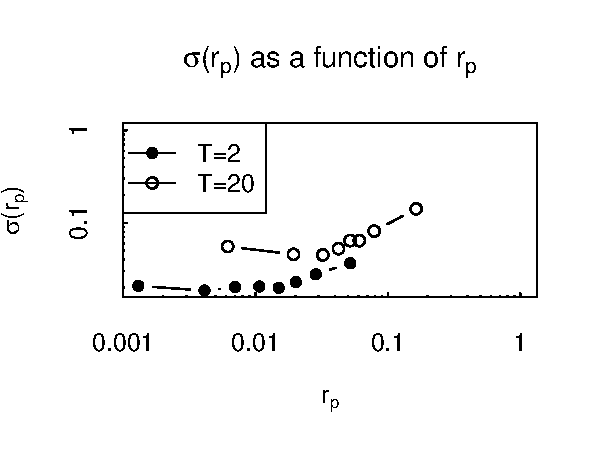
\includegraphics{figs/scaling-plot-1.pdf}
\caption{\label{fig:scaling-plot}The scaling factor \(\sigma(r_p)\) as a function of \(r_p\). The approximate linear dependency is confirmed by the calculation.}
\end{figure}

Finally, it should be noted that the scaling factor \(\sigma(r_p)\) does not
transform returns into independent random variables:
Figure~ \ref{fig:acf} displays
the autocorrelation of the scaled return and of its absolute value. This
observation should not come as a surprise, as volatility is commonly
modeled by an autoregressive process, and not by a function of the
previous observation alone.

\begin{Shaded}
\begin{Highlighting}[]
\NormalTok{bins }\OtherTok{\textless{}{-}} \FunctionTok{make.bins}\NormalTok{(r.QQQ, }\AttributeTok{NBIN=}\NormalTok{nb, }\AttributeTok{model=}\StringTok{\textquotesingle{}abs\textquotesingle{}}\NormalTok{, params)}
\FunctionTok{par}\NormalTok{(}\AttributeTok{mar=}\FunctionTok{c}\NormalTok{(}\DecValTok{4}\NormalTok{,}\DecValTok{4}\NormalTok{,}\FloatTok{0.1}\NormalTok{,}\FloatTok{0.1}\NormalTok{))}
\FunctionTok{acf}\NormalTok{(bins}\SpecialCharTok{$}\NormalTok{r.sc)}
\FunctionTok{acf}\NormalTok{(}\FunctionTok{abs}\NormalTok{(bins}\SpecialCharTok{$}\NormalTok{r.sc))}
\end{Highlighting}
\end{Shaded}

\begin{figure}[H]
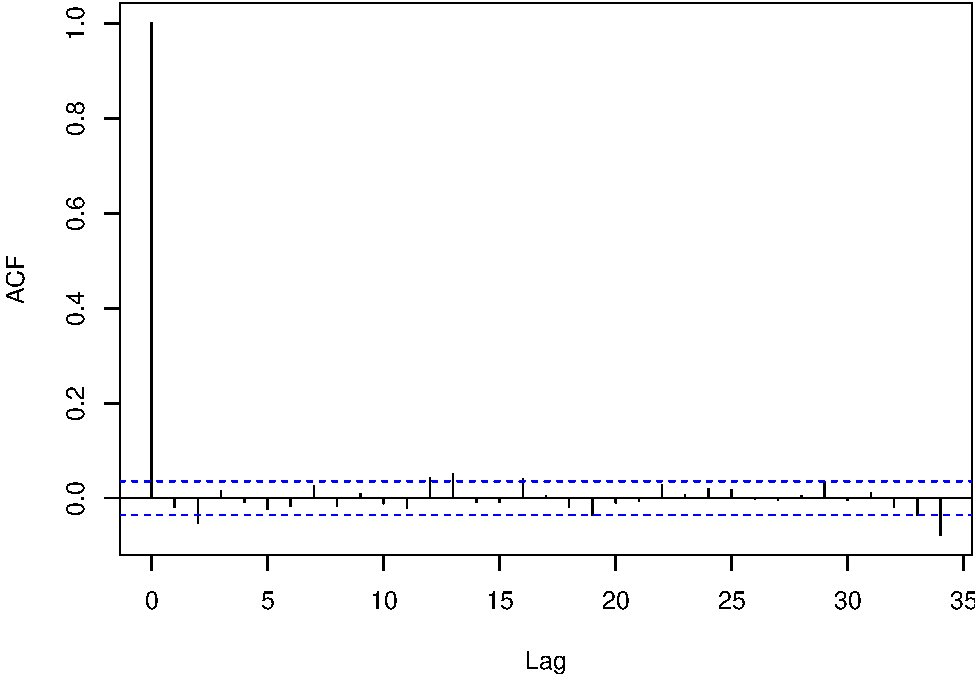
\includegraphics[width=0.5\linewidth]{figs/acf-1} 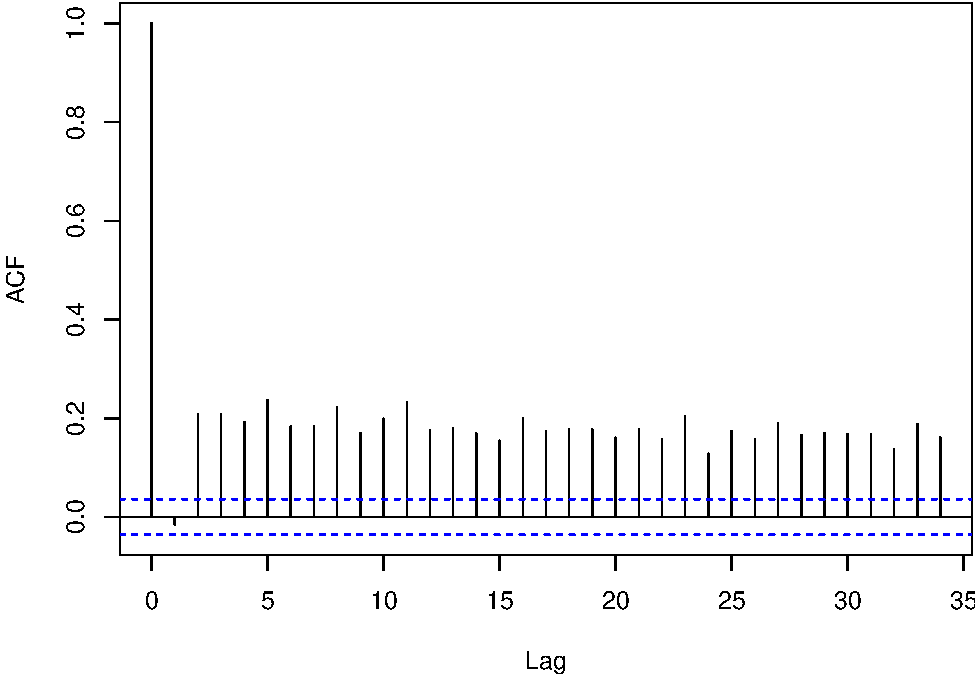
\includegraphics[width=0.5\linewidth]{figs/acf-2} \caption{Autocorrelation of $r_t/\sigma(r_p)$ and $|r_t|/\sigma(r_p)$. QQQ return serie, sampling $T=2$}\label{fig:acf}
\end{figure}

The effect of scaling can be measured by comparing Figure \ref{fig:acf} to the same calculation, performed on the original return serie. Scaling by \(\sigma(r_p)\) reduces the autocorrelation of absolute return, but does not completely cancel it.

\begin{Shaded}
\begin{Highlighting}[]
\FunctionTok{par}\NormalTok{(}\AttributeTok{mar=}\FunctionTok{c}\NormalTok{(}\DecValTok{4}\NormalTok{,}\DecValTok{4}\NormalTok{,}\FloatTok{0.1}\NormalTok{,}\FloatTok{0.1}\NormalTok{))}
\FunctionTok{acf}\NormalTok{(r.QQQ)}
\FunctionTok{acf}\NormalTok{(}\FunctionTok{abs}\NormalTok{(r.QQQ))}
\end{Highlighting}
\end{Shaded}

\begin{figure}[H]
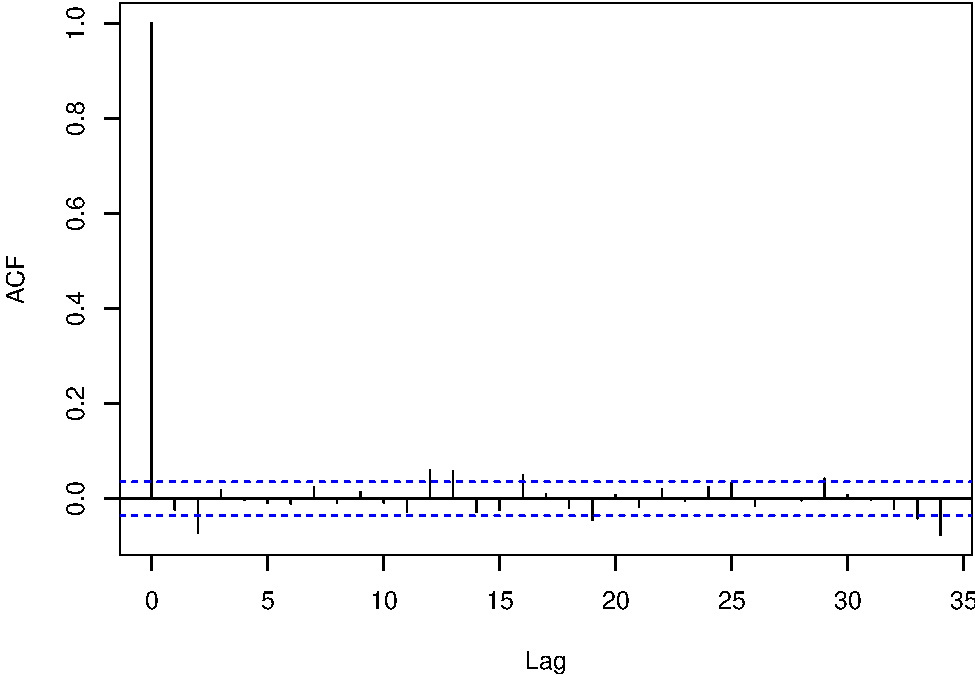
\includegraphics[width=0.5\linewidth]{figs/acf2-1} 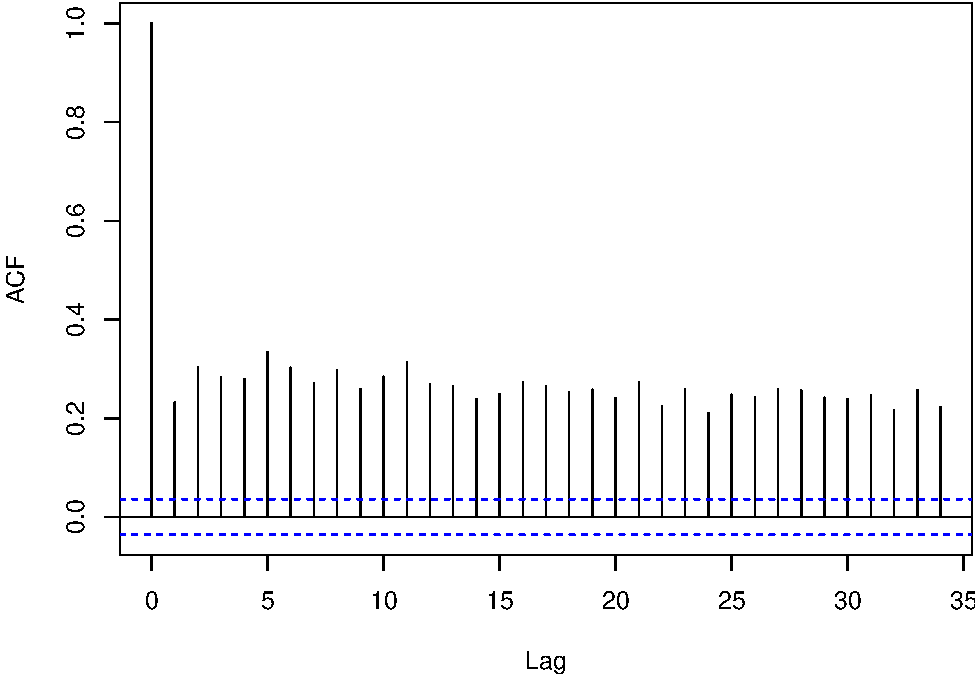
\includegraphics[width=0.5\linewidth]{figs/acf2-2} \caption{Autocorrelation of $r_t$ and $|r_t|$. QQQ return serie, sampling $T=2$}\label{fig:acf2}
\end{figure}

\hypertarget{conclusion}{%
\section{Conclusion}\label{conclusion}}

Scaling return series by a factor which is a function of the absolute value of return in the previous period provides a model for ``fat tails,'' but only partially captures the volatility clustering feature of financial time series.

\hypertarget{bibliography}{%
\section*{Bibliography}\label{bibliography}}
\addcontentsline{toc}{section}{Bibliography}

\hypertarget{refs}{}
\begin{CSLReferences}{1}{0}
\leavevmode\hypertarget{ref-Chen-2008}{}%
Chen, K., Jayaprakash, C., \& Yuan, B. (2008). {Conditional Probability as a Measure of Volatility Clustering in Financial Time Series}. \emph{Physica A}, 1--5. \url{http://arxiv.org/abs/0503157v2}

\leavevmode\hypertarget{ref-Clauset2009}{}%
Clauset, A., Shalizi, C. R., \& Newman, M. E. J. (2009). {Power-law distributions in empirical data}. \emph{SIAM Review}, \emph{51(4)}, 661--703.

\leavevmode\hypertarget{ref-Cont2001}{}%
Cont, R. (2001). {Empirical properties of asset returns: stylized facts and statistical issues}. \emph{Quantitative Finance}, \emph{1}, 223--236. \url{http://citeseerx.ist.psu.edu/viewdoc/summary?doi=10.1.1.16.5992}

\leavevmode\hypertarget{ref-Gopikrishnana1998}{}%
Gopikrishnan, P., Meyer, M., Amaral, L. A. N., \& Stanley, H. E. (1998). {Inverse cubic law for the distribution of stock price variations}. \emph{The European Physical Journal B}, \emph{3}, 139--140.

\leavevmode\hypertarget{ref-Williamson2013}{}%
Williamson, S. H. (2013). \emph{{Daily Closing Values of the DJA in the United States, 1885 to Present}}. \url{http://www.measuringworth.com/DJA/}

\end{CSLReferences}

\end{document}
